\section{Ether}
\label{sec:ether}
%\fbox{Responsible: UNEW, Provisional date: Nov 2016}

\subsection{Example Description}
\label{sec:ether_desc}

This example explores ways to model network communications between controllers. This involves passing messages ---VDM values encoded as strings--- from a model called \emph{Sender} to a model called \emph{Receiver}. This is either done directly, as illustrated in Figure~\ref{fig:send_rec}, or via a third model called the \emph{Ether}, as illustrated in Figure~\ref{fig:send_ether_rec}.

While this example demonstrates that direct connection is possible, for multi-models with large numbers of connected controllers (for example swarms or cooperative vehicles) it becomes unwieldy. This example includes an Ether model, which represents an abstract communication mechanism, that handles message passing between the Sender and Receiver. This Ether can be used in other models.

The introduction of a model of communications also permits a range of realistic and faulty behaviours to be introduced, such as message delay, duplication, and loss. The ether pattern which this example implements is described in greater detail in Deliverable D3.3a~\cite{INTOCPSD3.3a}, and includes a discussion of realistic and faulty behaviour.

\begin{figure}[h]
\begin{center}
\subfigure[Sender and Receiver connected directly]
{
     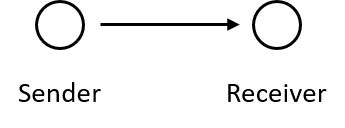
\includegraphics[scale=0.5]{ether/send_rec}
      \label{fig:send_rec}
}
\hspace{2em}\subfigure[Sender and Receiver connected via the Ether]
{
     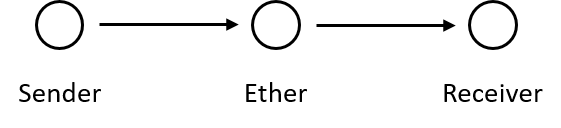
\includegraphics[scale=0.5]{ether/send_ether_rec}
      \label{fig:send_ether_rec}
}
\caption{Topology of the `Direct' and `Ether' multi-models.}
\label{fig:ether_topology}
\end{center}
\end{figure}

\subsection{Usage}
\label{sec:ether_usage}

The example is available from the INTO-CPS application menu at \emph{File > Import Example Project} or at  \url{https://github.com/into-cps/case-study\_ether} in the \emph{master} branch. There are several subfolders for the various elements: \texttt{FMU} -- contains the various FMUs of the study; \texttt{Models} -- contains the constituent models defined using the INTO-CPS simulation technologies; \texttt{Multi-models} -- contains the multi-model definitions and co-simulation configurations -- with Direct and Ether configurations.

The \texttt{case-study\_ether folder} can be opened in the INTO-CPS application to run various co-simulation experiments. To run a simulation, expand the emph{Direct} or emph{Ether} models, then open the \emph{co-sim\_direct} or {co-sim\_ether} experiments and click \emph{Simulate}. Section~\ref{sec:ether_into_analysis} below gives some suggestions of how to explore the multi-model.

%\textbf{Warning!} Values printed from Overture FMUs are not visible in the COE status window in the INTO-CPS Application version 2.1.0 or below.

%\subsection{INTO-CPS Technology}
%\label{sec:ether_into}

%\subsection{INTO-CPS SysML profile}
%\label{sec:ether_into_sys}

\subsection{Multi-model}
\label{sec:ether_into_mm}

\subsubsection{Models}

There are three models in this example, all of which are DE models written in VDM:

\begin{description}
  \item[Sender:] This model has a single output port called \texttt{out}, of type \texttt{String}. The \texttt{Controller} class generates random messages every 0.1 seconds, and passes them to the output port. Each message consists of three integers in the range (0,10), and are converted to a string representation using the \texttt{VDMUtil} standard library. The time and content of each message is printed to the console.
  \item[Receiver:] This model has a single input port called \texttt{iin}, of type \texttt{String}. The \texttt{Controller} class listens for messages on the input port and attempts to convert message strings back to a VDM type representation using the \texttt{VDMUtil} standard library. Empty strings are often received at the start of co-simulation, and these are ignored. If conversion is successful, the time and content of the message is printed to the console.
  \item[Ether:] This model represents an abstract communication medium. It has an input port called \texttt{sender} and an output port called \texttt{receiver}, both of type \texttt{String}. The \texttt{Ether} class passed strings from the \texttt{sender} port to the \texttt{receiver} port. Although in this example only one message will be received at a time, in general there may be multiple messages for the same destination during a single update, so the \texttt{Ether} class collects messages in a list and passes on a string of strings that the destination (i.e.\ in this case Receiver) must decode.

      The connections in the \texttt{Ether} class are determined by the values passed to the constructor, which is called in the \texttt{System} class. The constructor takes a map of named input ports, a map of named output ports and a set of pairs indicating which inputs are connected to which outputs. The \texttt{Ether} class does not examine the value of the messages that it passes. This model can be reused in other multi-models where message-based communications between models are required.
\end{description}

\subsubsection{Configuration}

There are two multi-model configurations included in the example:

\begin{description}
  \item[Direct] In this configuration, the \texttt{Sender.out} port is connected directly to the \texttt{Receiver.in} port.
  \item[Ether] In this configuration, the \texttt{Sender.out} port is connected to the \texttt{Ether.sender} port and the \texttt{Sender.reciever} port is connected to the \texttt{Receiver.in} port.
\end{description}

These two different configurations allow exploration of the consequences of introducing the Ether FMU. The Sender model does not need to know if it is connected to the Ether or not. Since the Ether allows one-to-many communications, it passes lists of values, so the Receiver must check whether it received a single value from the Sender directly, or a list containing a single value via the Ether. This could be avoided in this example by letting the Ether assume that there is only one connection, but would make the Ether less general. The included implementation means that the Ether can be used directly in other multi-models --- only the \texttt{HardwareInterface} class and called to the constructor of \texttt{Ether} would need to be changed for the context of the new model.

\subsection{Co-simulation}
\label{sec:ether_into_co}

The simulation time for the multi-model is set to one second, which is sufficient to see the behaviour of the system. During this time, 10 messages are sent from the Sender.  Not all messages are received by the Receiver since at least one extra update cycle is needed to process the final message, or final two messages in the case of communication via the Ether.

\subsection{Analyses and Experiments}
\label{sec:ether_into_analysis}


\subsubsection{Sample Experiments}
\label{sec:ether_exp}

The following experiments are instructive in demonstrating the effects on introducing the Ether and the effects of the relative speeds up the \emph{Sender}, \emph{Ether} and \emph{Receiver} on messages. All three FMUs print messages and times to the COE console.

\begin{enumerate}
  \item Run the \emph{Direct} co-simulation and observe that messages arrive at Receiver one step (0.1 seconds) later. Run the \emph{Ether} co-simulation and observe that messages arrive two steps (0.2 seconds) later.
  \item Change the frequency of the Ether to 20Hz or higher. Run the \emph{Ether} co-simulation and observe that messages arrive at Receiver one step (0.1 seconds) later. This is because the Ether can now update in between steps of the Receiver.
  \item Set the Ether back to 10Hz and change the frequency of the Sender to 20Hz or higher. Run the \emph{Ether} co-simulation and note how messages are not lost because they are changed by the Sender before they are read by the Ether.
  \item Set the Sender back to 10Hz and change the frequency of the Receiver to 20Hz or higher. Run the \emph{Ether} co-simulation and note how messages are now duplicated because the Receiver is reading them twice or more.
\end{enumerate}

If elimination of message loss or duplication is important in a multi-model,
the description of the ether pattern in Deliverable D3.3a~\cite{INTOCPSD3.3a} gives some initial guidance on overcoming such problems by introducing extra logic to give quality of service (QoS) guarantees in message-passing. 


\subsubsection{Test Automation and Model Checking}
\label{sec:ether_ta}
\graphicspath{ {./ether/TA/} }

Our model for test automation is different from that for Multi-model and analysis in the following aspects.
\begin{itemize}
    \item Our test model aims for model network communications between multiple controllers through an intermediate \emph{Ether}. The \emph{Ether} is regarded as a shared medium between controllers to dispatch packages from multiple sources to multiple targets. Therefore, we do not need all controllers connected to each other directly and the direct connection mode between controllers is not taken into account in our test model.
    \item Current Multi-model configuration \B{Ether} includes only one \T{Sender} and one \T{Receiver}. In order to be used as a communication medium in the UAV swarm pilot study in Section~\ref{sec:uavswarm}, the \emph{Ether} model should support more senders and receivers. Our test model supports two controllers to be connected through the \emph{Ether}, and each controller is composed of a sender and a receiver to allow it to communicate with others bidirectionally.
    \item For Co-Simulation, these controllers could be in different FMUs. Then the \emph{Ether} should provide the capability to dispatch packages from sources to destinations according to their targets. For instance, one central controller would send a command to the controller one at a specific time, then later it would send another command to the controller two. We introduce a new package structure (as shown in Section~\ref{sssec:ether_encoding}) which is composed of an address part and a payload part. Therefore, the \emph{Ether} is able to dispatch packages by the addresses that are encoded in the packages. In particular, it supports broadcast and unicast.
    \item The model for Multi-model and analysis has messages encoded in strings. But due to the fact that RT-Tester is not able to parse string or array in test models, we are not able to model variable-length strings in test models. The encoding mechanism in Section~\ref{sssec:ether_encoding} is an example to encode a string (up to 5 Base64 characters) into a 32-bit integer. We allow different applications can have different encoding mechanisms. As an example, the test model in the UAV swarm study uses three doubles for its payload and each double means a position or velocity in one of three axes (X, Y and Z). However, for this \emph{Ether} pilot study, the test model will not look into the inside of payloads and it just uses an integer for illustration.
\end{itemize}

Subsequently, we present the test model in SysML. Then model checking is applied to check a number of properties of the test model. Finally a SUT is implemented manually and test automation is applied to test whether the SUT is a correct implementation of the test model.

\paragraph{Test Model [Ether mode]}
Our test model connected two controllers (or FMUs, here we call it \emph{End}) through a \emph{Ether}. The interfaces between the \emph{TestEnvironment} and the \emph{SystemUnderTest} are the packages that two \emph{Ends} would send and receive.

\subparagraph{String Encoding}
\label{sssec:ether_encoding}
A package is composed of two parts: address and payload. Each of them is encoded in one integer (32-bit). 
\begin{itemize}
    \item Address (32-bit integer): the high 24 bits are always 0, the low 8 bits are split into two 4-bit parts (one for the destination port and one for the source port)
        \begin{itemize}
            \item 0xF: for broadcast;
            \item 0x1-0xE: port 1 - port 15;
            \item 0x0: no message signal (used for the polling method to identify a valid package).
        \end{itemize}
    \item Payload (32-bit integer): the highest two bits are reserved, other 30 bits consist of five 6-bit parts (each encodes a Base64 character)
        \begin{itemize}
            \item Base64: 64 characters (26 uppercase alphabet letters [A-Z], 26 lowercase alphabet letters [a-z], 10 digits [0-9], '+' and '/'),
            \item up to five characters in a string.
        \end{itemize}
\end{itemize}

Finally, it supports
\begin{itemize}
    \item up to 15 incoming ports and 15 outgoing ports, and each FMU (or end) has a paired incoming and outgoing ports,
    \item up to 15 FMUs connected,
    \item the paired ports have the same and unique id,
    \item the destination address of an input pair can be its paired port (send a message to itself),
    \item up to 5 characters in the payload of each package.
\end{itemize}

\subparagraph{Inputs and Outputs}
Inputs and outputs of the test model are shown in Figure~\ref{fig:ether-inouts}.
\begin{figure}[htb!]
    \centering
    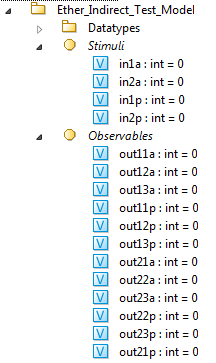
\includegraphics[width=0.4\textwidth]{ether_inouts}
    \caption{Input and Output Variables of Ether}
    \label{fig:ether-inouts}
\end{figure}

The \emph{SystemUnderTest} receives the following inputs (stimuli) from the \emph{TestEnvironment}:
\begin{itemize}
    \item $in1a$ and $in1p$: address and payload of the incoming package in \emph{Ether} from End 1, 
    \item $in2a$ and $in2p$: address and payload of the incoming package in \emph{Ether} from End 2. 
\end{itemize}

The \emph{SystemUnderTest} provides the following observable outputs to the \emph{TestEnvironment}:
\begin{itemize}
    \item $out11a$ and $out11p$: address and payload of the first outgoing package in \emph{Ether} to End 1,
    \item $out12a$ and $out12p$: address and payload of the second outgoing package in \emph{Ether} to End 1,
    \item $out13a$ and $out13p$: address and payload of the third outgoing package in \emph{Ether} to End 1,
    \item $out21a$ and $out21p$: address and payload of the first outgoing package in \emph{Ether} to End 2,
    \item $out22a$ and $out22p$: address and payload of the second outgoing package in \emph{Ether} to End 2,
    \item $out23a$ and $out23p$: address and payload of the third outgoing package in \emph{Ether} to End 2. 
\end{itemize}

\subparagraph{Other Interfaces}
Other interfaces, as shown in Figure~\ref{fig:ether-other-ifs}, are used in the \emph{SystemUnderTest} for connections between the \emph{Ends} and the \emph{Ether}.
\begin{figure}[htb!]
    \centering
    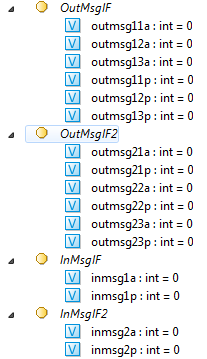
\includegraphics[width=0.4\textwidth]{ether_other_ifs}
    \caption{Other Interfaces of Ether}
    \label{fig:ether-other-ifs}
\end{figure}

\begin{itemize}
    \item $InMsgIF$ and $OutMsgIF$: the incoming and outgoing interfaces between the \emph{End1} and the \emph{Ether}, 
    \item $InMsgIF2$ and $OutMsgIF2$: the incoming and outgoing interfaces between the \emph{End2} and the \emph{Ether}.
\end{itemize}

\subparagraph{SystemUnderTest Architecture Diagram}
The system architecture diagram of the \emph{SystemUnderTest} is shown in Figure~\ref{fig:ether-sut-sad}. It consists of two \emph{Ends}: \emph{End1} and \emph{End2}, and one \emph{Ether}.
\begin{figure}[htb!]
    \centering
    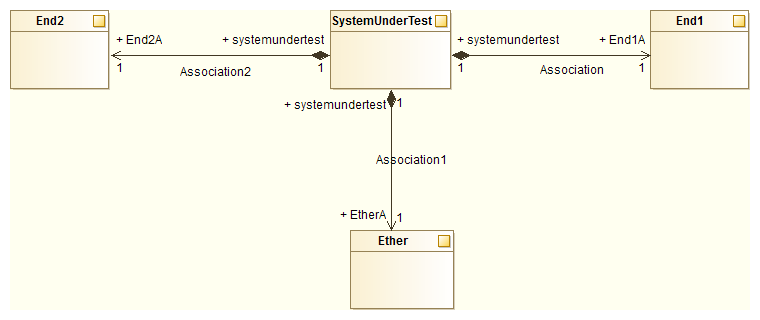
\includegraphics[width=0.7\textwidth]{ether_sut_sad}
    \caption{Ether Architecture Diagram}
    \label{fig:ether-sut-sad}
\end{figure}

\subparagraph{SystemUnderTest Connection Diagram}
The connection diagram of the \emph{SystemUnderTest} is illustrated in Fig~\ref{fig:ether-cd}. Both \emph{End1} and \emph{End2} are connected to the \emph{Ether}, but they are not connected directly. Therefore, a package that is sent from the \emph{End1} to the \emph{End2} would transmit to the \emph{Ether} at first, then dispatch to the \emph{End2} by the \emph{Ether}. 

\begin{figure}[htb!]
    \centering
    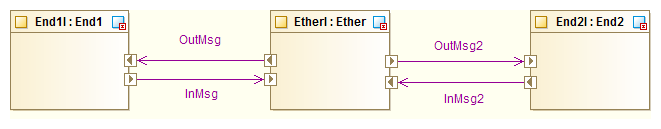
\includegraphics[width=0.8\textwidth]{ether_sut_cd}
    \caption{Ether Connection Diagram}
    \label{fig:ether-cd}
\end{figure}

\subparagraph{End1 State Machine Diagram}
The behaviour of the \emph{End1} is specified in the state machine diagram shown in Figure~\ref{fig:ether-sut-end1-sm}. It merely copies the input packages from the \emph{TestEnvironment} to the \emph{Ether} and the output packages from the \emph{Ether} to the \emph{TestEnvironment}.

\begin{figure}[htb!]
    \centering
	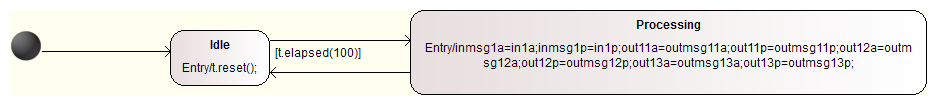
\includegraphics[width=0.7\textwidth]{ether_sut_end1_sm}
    \caption{End1 State Machine Diagram}
    \label{fig:ether-sut-end1-sm}
\end{figure}

\subparagraph{End2 State Machine Diagram}
Similarly, the state machine diagram of the \emph{End2} is displayed in Figure~\ref{fig:ether-sut-end2-sm}.

\begin{figure}[htb!]
    \centering
	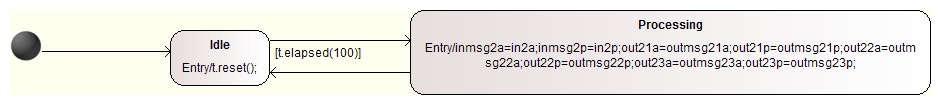
\includegraphics[width=0.8\textwidth]{ether_sut_end2_sm}
    \caption{End2 State Machine Diagram}
    \label{fig:ether-sut-end2-sm}
\end{figure}

\subparagraph{Ether State Machine Diagram}
The behaviour of the \emph{Ether} is specified in the state machine diagram shown in Figur~\ref{fig:ether-sut-ether-sm}. Basically, it checks the incoming packages from the \emph{End1} and the \emph{End2}, and then dispatches them to their corresponding output ends according to the address in each package.

\begin{figure}[htb!]
    \centering
	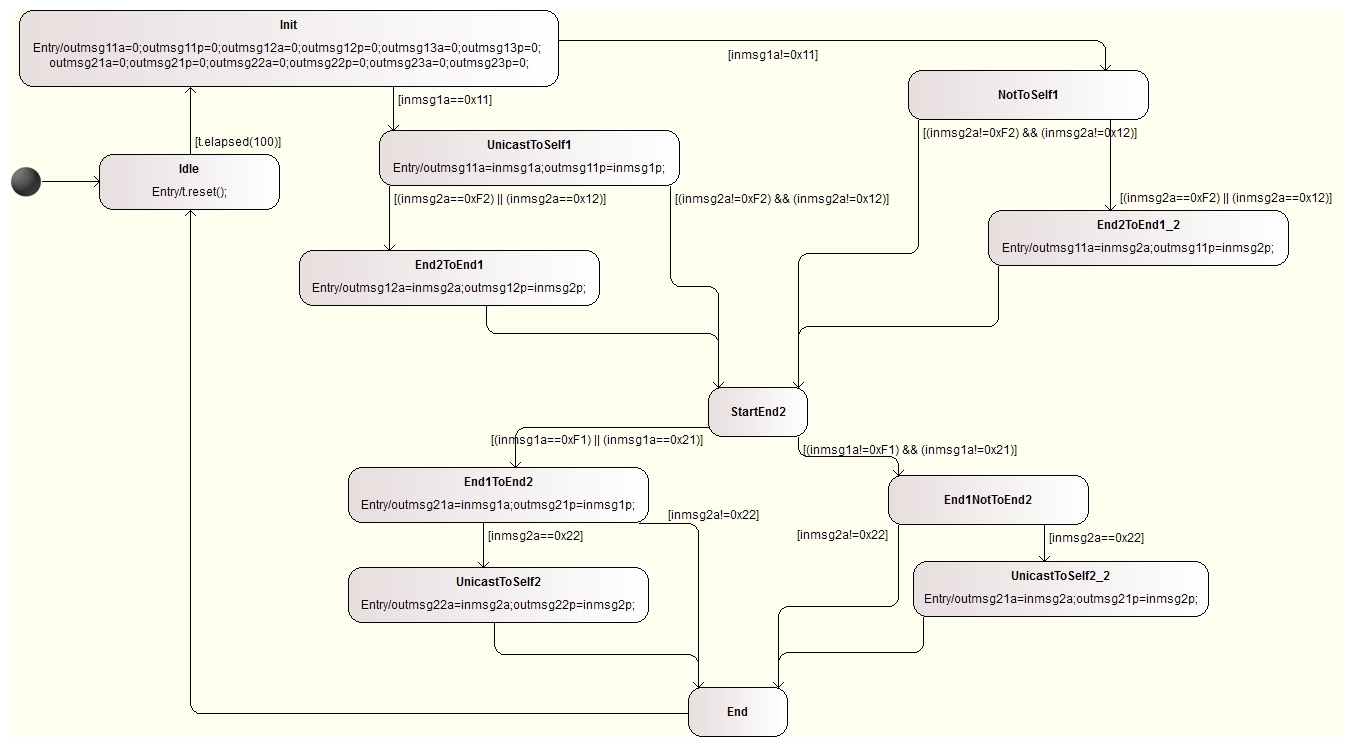
\includegraphics[width=1.0\textwidth]{ether_sut_ether_sm}
    \caption{Ether State Machine Diagram}
    \label{fig:ether-sut-ether-sm}
\end{figure}

\subparagraph{Test Input Simulation} We use a state machine to specify the input sequence in the \T{TestEnvironment} of the test model. The diagram is shown in Figure~\ref{fig:ether-te-sim-sm}. This state machine simulates all combinations of incoming packages from the \emph{End1} and \emph{End2} in terms of package addresses. 

\begin{figure}[htb!]
    \centering
	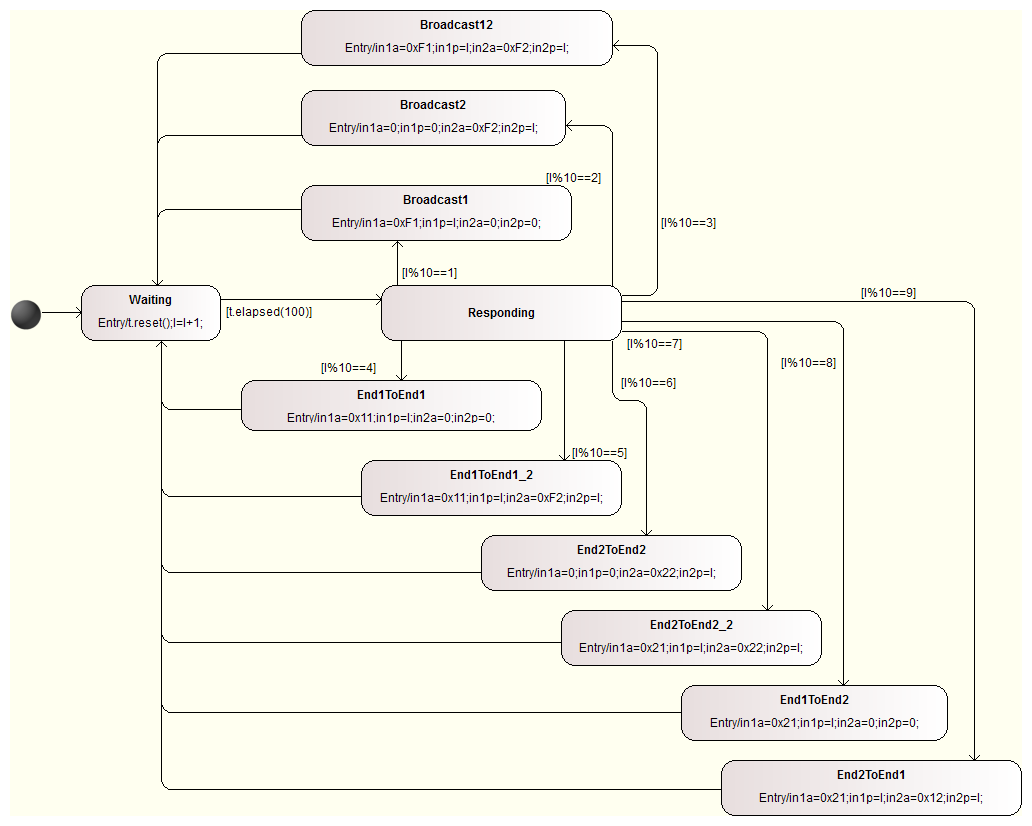
\includegraphics[width=1.0\textwidth]{ether_te_sim_sm}
    \caption{Test Input Simulation State Machine Diagram}
    \label{fig:ether-te-sim-sm}
\end{figure}

\paragraph{Model Checking}

Model checking can be applied to the test model to check if it satisfies several properties. In order to use bounded model checking in the INTO-CPS app, we set the bounded steps ``BMC steps'' to 50. The properties below are checked to hold in 50 steps.

\begin{description}
    \item[P0] Livelock property by the \B{Check Mode} function on RT-Tester.
\begin{verbatim}
Check static model semantics ...done.
- IMR.SystemUnderTest.End1I... [PASS]
- IMR.SystemUnderTest.End2I... [PASS]
- IMR.SystemUnderTest.EtherI... [PASS]
- IMR.TestEnvironment.tesimulator... [PASS]
\end{verbatim}

    \item[P1] An \emph{End} would never receive a package with a wrong destination address.
\begin{verbatim}
Globally ([IMR.out11a != 33] && 
    [IMR.out11a != 34] && 
    [IMR.out21a != 17] && 
    [IMR.out21a != 18])
\end{verbatim}

    \item[P2] All controllers could be in the \emph{Idle} state at the same time.
\begin{verbatim}
Finally ([IMR.SystemUnderTest.End1I.End.Idle
    && IMR.SystemUnderTest.EtherI.Ether.Idle
    && IMR.SystemUnderTest.End2I.End.Idle])
\end{verbatim}

    \item[P3] A broadcast package would never be received by its source port.
\begin{verbatim}
Globally ([IMR.out11a != 241] && [IMR.out21a != 242])
\end{verbatim}
\end{description}

\paragraph{A Manual Implementation of SUT in C}
A SUT is implemented in C. And it is finally built and wrapped into a SUT FMU.

\paragraph{Test Results}

\subparagraph{Test Goals}
Our test goals configuration is displayed in Figure~\ref{fig:ether-ta-tr01-testgoal}. All basic control state coverage test cases and transition coverage test cases for three controllers are included, in the context of the \emph{TestEnvironment} simulation enabled. In addition, a user defined test case is presented to require the test lasting at least 1.5 seconds. The generated and solved input signals for the test goals are shown in Figure~\ref{fig:ether-ta-tr01-signal-inputs-tp1} and Figure~\ref{fig:ether-ta-tr01-signal-inputs-tp2}.

\begin{figure}[htb!]
	\centering
	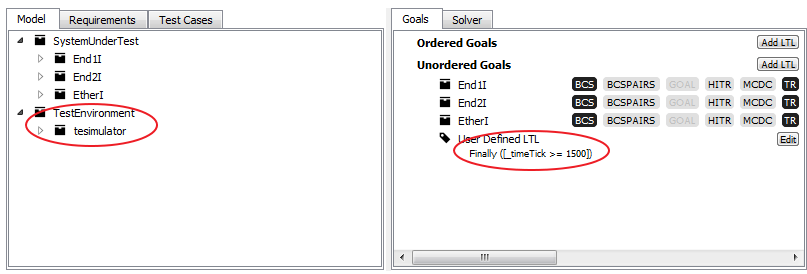
\includegraphics[width=1.0\textwidth]{tr01/tr01-testgoals}
	\caption{Test Goals Configuration}
	\label{fig:ether-ta-tr01-testgoal}
\end{figure}

\begin{figure}[htb!]
    \centering
	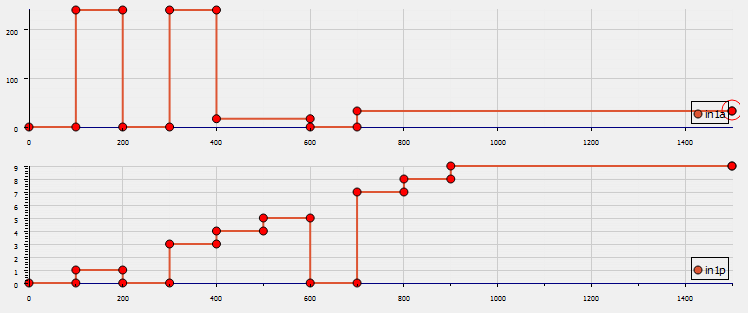
\includegraphics[width=1.0\textwidth]{tr01/tr01-signal-inputs-tp1}
    \caption{Input Signals of \emph{End1}}
    \label{fig:ether-ta-tr01-signal-inputs-tp1}
\end{figure}

\begin{figure}[htb!]
    \centering
	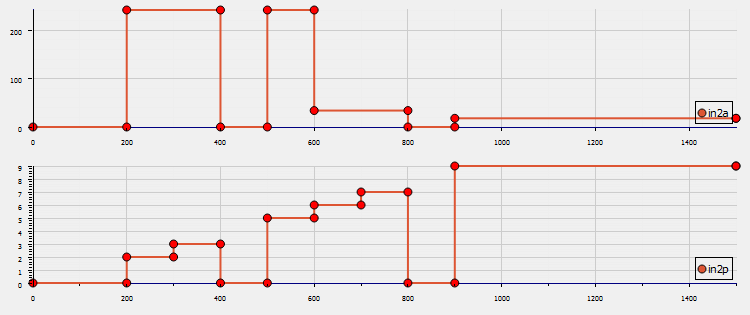
\includegraphics[width=1.0\textwidth]{tr01/tr01-signal-inputs-tp2}
    \caption{Input Signals of \emph{End2}}
    \label{fig:ether-ta-tr01-signal-inputs-tp2}
\end{figure}

The input address signals for both \emph{End1} and \emph{End2} (where the payloads are excluded) are marked and illustrated in Figure~\ref{fig:ether-ta-tr01-signal-inputs}.

\begin{figure}[htb!]
    \centering
	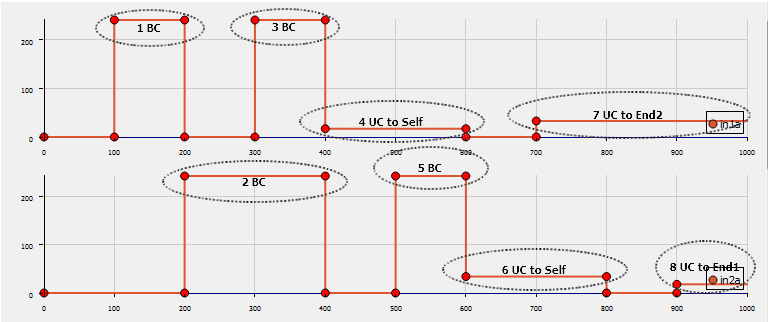
\includegraphics[width=1.0\textwidth]{tr01/tr01-signal-inputs}
    \caption{Input Address Signals}
    \label{fig:ether-ta-tr01-signal-inputs}
\end{figure}

\subparagraph{\emph{TP-00} vs. \emph{Simulation}}
The \emph{TP-00} is a test procedure in RT-Tester that provides test inputs and checks expected results, while \emph{Simulation} is a SUT test procedure created from the same test model as the \emph{TP-00}. Our test results show all these test cases are with \T{PASS} or \T{INCONCLUSIVE} verdicts. 

\subparagraph{\emph{TP-00} vs. \emph{SUT}}
This is to test if our manually implemented SUT is a correct implementation of the test model or not. Our test results show all these test cases are with \T{PASS} or \T{INCONCLUSIVE} verdicts. Corresponding to the inputs shown in Figure~\ref{fig:ether-ta-tr01-signal-inputs-tp1} and Figure~\ref{fig:ether-ta-tr01-signal-inputs-tp2} as well as the marked input signals in Figure~\ref{fig:ether-ta-tr01-signal-inputs}, the output signals for the \emph{End1} and the \emph{End2} are illustrated in Figure~\ref{fig:ether-ta-tr01-signal-output-1} and Figure~\ref{fig:ether-ta-tr01-signal-output-2} respectively.

\begin{figure}[htb!]
    \centering
	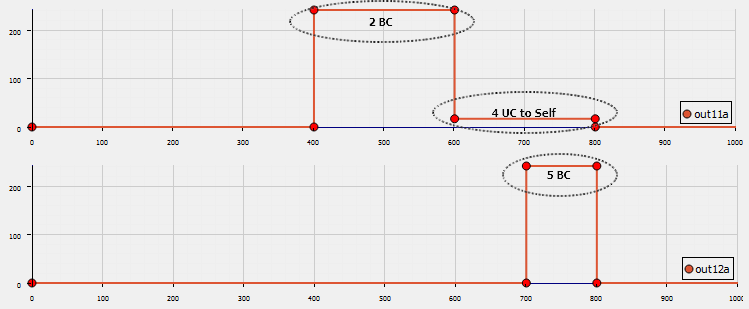
\includegraphics[width=1.0\textwidth]{tr01/tr01-signal-output-1}
    \caption{Output Signals of \emph{End1}}
    \label{fig:ether-ta-tr01-signal-output-1}
\end{figure}

\begin{figure}[htb!]
    \centering
	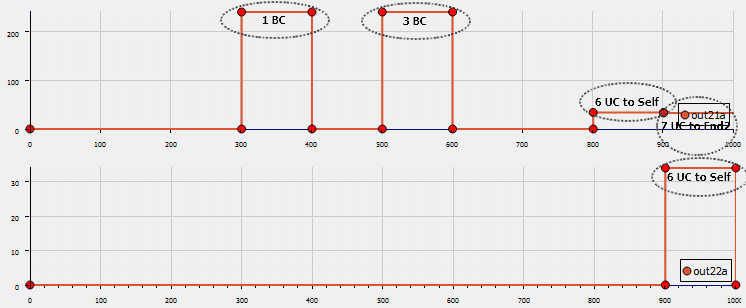
\includegraphics[width=1.0\textwidth]{tr01/tr01-signal-output-2}
    \caption{Output Signals of \emph{End2}}
    \label{fig:ether-ta-tr01-signal-output-2}
\end{figure}

 Our test results show all these test cases are with \T{PASS} or \T{INCONCLUSIVE} verdicts. These signals are described below with numbering.
\begin{itemize}
    \item 1. Broadcast from \emph{End1} ([100ms, 200ms]), 
        \begin{itemize}
            \item as shown in the outputs of \emph{End2} ([300, 400]),
            \item therefore, 200ms delay.
        \end{itemize}
    \item 2. Broadcast from \emph{End2} ([200, 400]), 
        \begin{itemize}
            \item as shown in the outputs of \emph{End1} ([400, 600]).
        \end{itemize}
    \item 3. Broadcast from \emph{End1} ([300, 400]), 
        \begin{itemize}
            \item as shown in the outputs of \emph{End2} ([500, 600]).
        \end{itemize}
    \item 4. Unicast from \emph{End1} to \emph{End1} ([400, 600]), 
        \begin{itemize}
            \item as shown in the output (\verb+out11a+) of \emph{End1} ([600, 800]).
        \end{itemize}
    \item 5. Broacast from \emph{End2} ([500, 600]), 
        \begin{itemize}
            \item as shown in the output (\verb+out12a+) of \emph{End1} ([700, 800]).
        \end{itemize}
    \item 6. Unicast from \emph{End2} to \emph{End2} ([600, 800]), 
        \begin{itemize}
            \item as shown in the output (\verb+out21a+) of \emph{End2} ([800, 900]),
            \item and the output (\verb+out22a+) of \emph{End2} ([900, 1000]).
        \end{itemize}
    \item 7. Unicast from \emph{End1} to \emph{End2} ([700, \ldots]), 
        \begin{itemize}
            \item as shown in the output (\verb+out21a+) of \emph{End2} ([900, 1000]).
        \end{itemize}
    \item 8. Unicast from \emph{End2} to \emph{End1} ([900, 1000]), \ldots
\end{itemize}

These behaviours are expected in our test model.
